% -*- TeX:de -*-
\NeedsTeXFormat{LaTeX2e}
\documentclass[12pt,a4paper]{article}
\usepackage[german]{babel} % german text
\usepackage[DIV12]{typearea} % size of printable area
\usepackage[T1]{fontenc} % font encoding
%\usepackage[latin1]{inputenc} % most likely on Windows
\usepackage[utf8]{inputenc} % probably on Linux
\usepackage{multicol}

% PLOTTING
\usepackage{pgfplots} 
\usepackage{pgfplotstable}
\usepackage{url}
\usepackage{graphicx} % to include images
\usepackage{tikz}
\usepackage{subfigure} % for creating subfigures
\usepackage{amsmath} % a bunch of symbols
\usepackage{amssymb} % even more symbols
\usepackage{booktabs} % pretty tables
\usepackage{makecell} % multi row table heading

% a floating environment for circuits
\usepackage{float}
\usepackage{caption}

%\newfloat{circuit}{tbph}{circuits}
%\floatname{circuit}{Schaltplan}

% a floating environment for diagrams
%\newfloat{diagram}{tbph}{diagrams}
%\floatname{diagram}{Diagramm}

\selectlanguage{german} % use german

\begin{document}








%%%% TO DO
%
% - - Shorty:
%
% - - Tabelle "Messwerte Linsenbrennweite"
%		bitte bei jedem neuen e eine trennlinie... bin zu deppert ^^

% - - Patrick
%




%%%%%%% DECKBLATT %%%%%%%
\thispagestyle{empty}
			\begin{center}
			\Large{Fakultät für Physik}\\
			\end{center}
\begin{verbatim}


\end{verbatim}
							%Eintrag des Wintersemesters
			\begin{center}
			\textbf{\LARGE WS 2013/14}
			\end{center}
\begin{verbatim}


\end{verbatim}
			\begin{center}
			\textbf{\LARGE{Physikalisches Praktikum\\ für das Bachelorstudium}}
			\end{center}
\begin{verbatim}




\end{verbatim}

			\begin{center}
			\textbf{\LARGE{PROTOKOLL}}
			\end{center}
			
\begin{verbatim}





\end{verbatim}

			\begin{flushleft}
			\textbf{\Large{Experiment (Nr., Titel):}}\\
							%Experiment Nr. und Titel statt den Punkten eintragen
			\LARGE{PW9 Gleichstrom}	
			\end{flushleft}

\begin{verbatim}

\end{verbatim}	
							%Eintragen des Abgabedatums, oder des Erstelldatums des Protokolls
			\begin{flushleft}
			\textbf{\Large{Datum:}} \Large{21.11.2013}
			\end{flushleft}
			
\begin{verbatim}
\end{verbatim}
							%Namen der Protokollschreiber
		\begin{flushleft}
			\textbf{\Large{Namen:}} \Large{Patrick Braun, Johannes Kurz}
			\end{flushleft}

\begin{verbatim}


\end{verbatim}
							%Kurstag und Gruppennummer, zb. Fr/5
			\begin{flushleft}
			\textbf{\Large{Kurstag/Gruppe:}} \Large{DO/2}
			\end{flushleft}

\begin{verbatim}



\end{verbatim}
							%Name des Betreuers, das Praktikum betreute.
			\begin{flushleft}
			\LARGE{\textbf{Betreuer:}}	\Large{ Clemens Nagel }	
			\end{flushleft}

%%%%%%% DECKBLATT ENDE %%%%%%%
\pagebreak
\setlength{\columnsep}{20pt}
\begin{multicols}{2}

%%%%%%%%%%%%%%%%%%%%%%%%%%%%%%%%%%%%%%%%%%%%%%%%
%\end{multicols}
%\begin{figure}[H]
%	\centering
%	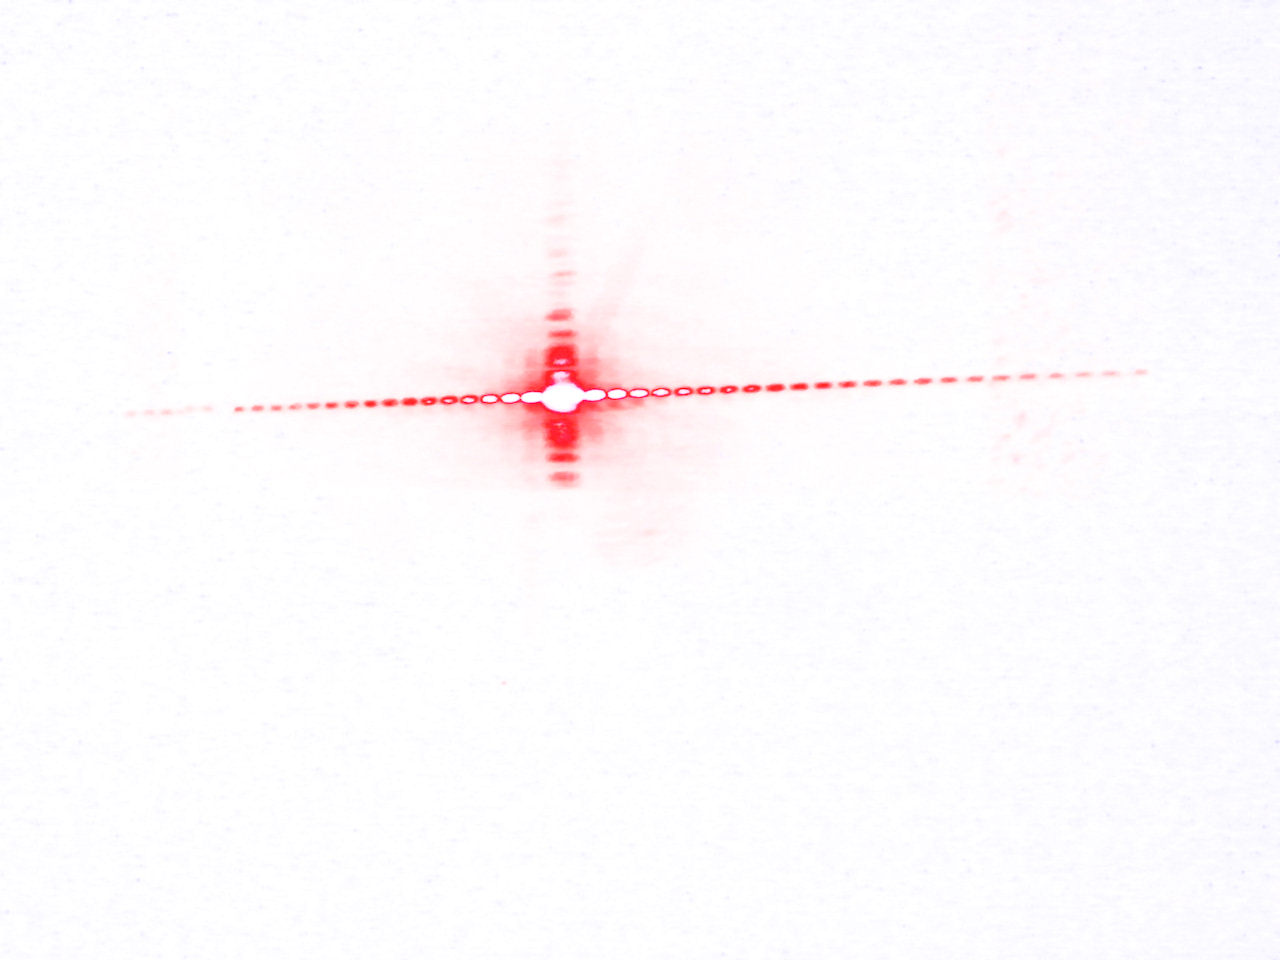
\includegraphics[scale=0.35]{./figure/beugung.png}
%	\caption{Beugungsmuster Einzelspalt (echtes Foto; schwarz durch weiß ersetzt)}
%	\label{fig:beugungsmuster}
%\end{figure}


%\begin{figure}[H]
%	\centering
%	\pgfplotstabletypeset[
%			columns={abstand, n},
%			col sep=&,
%			columns/abstand/.style={precision=2, zerofill, column name=\makecell{$Abstand$\\$(\pm 0.05)[mm]$} }, 
%			columns/n/.style={column name=\makecell{$n$\\$(Ordnung)$}, precision=0},
%			every head row/.style={before row=\hline,after row=\hline\hline},
%			every last row/.style={after row=\hline},
%			every first column/.style={column type/.add={|}{} },
%			every last column/.style={column type/.add={}{|} }
%			]{
%			abstand & n
%			12.9 & 1
%			24.45 & 2
%			37.40 & 3
%			49.35& 4
%			62.45 & 5
%			74.45 & 6
%			87.45 & 7
%			100.25 & 8
%			
%			}
%	\caption{Messwerte Einzelspalt}
%	\label{tab:werte_einzelspalt}
%\end{figure}
%


\section{Photovoltaische Solarzellen als Gleichstromquelle}
\subsection{Messwerte und Ergebnisse}

\subsection{Diskussion}
%%%%%%%%%%%%%%%%%%%%%%%%%%%%%%%%%%%%%%%%%%%%%%%%
\section{Widerstandsbestimmung mittel Wheatstone-Brücke}

Eine Möglichkeit, einen Widerstand zu messen, ohne mit 2 Messgeräten (und 2 Messunsicherheiten) Spannung und Strom zu bestimmen ist eine Wheatstone-Brückenschaltung.
\\
Der zu messende Widerstand (hier $R_x$) und 3 andere werden, paarweise parallel geschaltet, und innerhalb beider Zweige in Serie. 

Die beiden Zweige der Parallelschaltung werden durch ein Voltmeter verbunden, wie in Abb. \ref{fig:wheatstone_schaltplan} skizziert.



\begin{figure}[H]
	\centering
	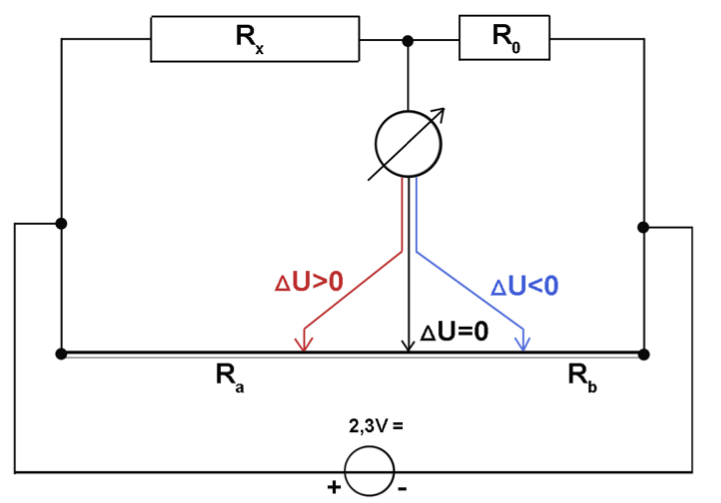
\includegraphics[scale=0.50]{./figure/wheatstone_schaltplan.png}
	\caption{Schaltskizze einer Wheatstonebrücke}
	\label{fig:wheatstone_schaltplan}
\end{figure}

An beiden Zweigen der Parallelschaltung liegt die gleiche Spannung an (Kirchhoff Schleifenregel). Diese teilt sich an den in Serie geschalteten Widerständen in derem Verhältnis auf.\\
Die Spannung im Messgerät ("Indikatorzweig") verschwindet genau dann, wenn die Verhältnisse der Widerstände an beiden Brückenzweigen gleich sind.

$$\frac{R_x}{R_0} = \frac{R_a}{R_b}$$
$$\Rightarrow R_x = R_0 \cdot \frac{R_a}{R_b}$$

Es genügt also, $R_0$ zu kennen, sowie das Verhältnis von $R_a$ zu $R_b$. Ihre Widerstandswerte sind nicht von Bedeutung.\\
\\
In diesem Versuch werden die WIderstände $R_a$,$R_b$ durch einen Draht realisiert, der an einer Längenskala befestigt ist, an der auch ein beweglicher Schleifer montiert ist. Durch diesen wird wird die Unterteilung in 2 Widerstände erzeugt (das Voltmeter ist am Schleifer angeschlossen).
\\
Da der Draht über die ganze Länge die gleiche Dicke hat, ist der Widerstand pro Längeneinheit überall gleich. Somit ist das Verhältnis der Drahtstücke, die durch den Schleifer getrennt werden gleichzeitig das Verhältnis der Widerstände.\\
Als $R_0$ wird eine Widerstandsdekade verwendet, auf der sich, in diskreten Schritten, Widerstände in von 1$ \Omega$ bis 10M$\Omega$ einstellen lassen
\\
Der Schleifer wird so lange verrückt, bis am Messgerät keine Spannung anliegt. Dann sind die Spannungsverhältnisse in beiden Zweigen gleich und der gesuchte Widerstand kann berechnet werden.\\
Es ist dabei eigentlich nicht notwendig, die Widerstandsdekade anders einzustellen. In der Diskussion wird jedoch näher erklärt, warum es sinnvoll ist, nicht das $R_a$-$R_b$-Verhältnis zu ändern, sondern $R_0$ anzupassen.

\subsection{Messwerte und Ergebnisse}

\subsection{Diskussion}
%%%%%%%%%%%%%%%%%%%%%%%%%%%%%%%%%%%%%%%%%%%%%%%%
\section{Reale Spannungsquelle}


\subsection{Messwerte und Ergebnisse}


\subsection{Diskussion}

%%%%%%%%%%%%%%%%%%%%%%%%%%%%%%%%%%%%%%%%%%

\section{Belasteter Spannungsteiler}

\subsection{Messwerte und Ergebnisse}


\subsection{Diskussion}

%%%%%%%%%%%%%%%%%%%%%%%%%%%%%%%%%%%%%%%%%%


\section{Quellen}
$[1]$ Leitfaden, \url{http://www.univie.ac.at/anfpra/neu1/pw/pw8/PW8.pdf}\\
$[2]$ Quecksilberdampflampe, \url{http://de.wikipedia.org/wiki/Quecksilberdampflampe}\\
%$[2]$

\end{multicols}


\end{document}